\documentclass[times,english,brazil,oneside,a4paper,fleqn]{ifes8}

\usepackage[utf8]{inputenc}
\usepackage[T1]{fontenc}
\usepackage{lastpage}           
\usepackage[alf]{abntex2cite}
\usepackage{microtype}          
\usepackage{morefloats}        
\usepackage{listings}
\usepackage{xcolor}
\usepackage{tikz}
\usepackage{hyperref}
\usetikzlibrary[topaths]
\usepackage{mathtools}
\usepackage[final]{pdfpages}
\usepackage{caption}
\usepackage{subcaption}
\usepackage{multirow}
\usepackage{hhline}
\usepackage{boxhandler}
\usepackage[normalem]{ulem}
\usepackage{dirtytalk}
\usepackage{float}
\usepackage{siunitx}
\usepackage{svg}
\usepackage[none]{hyphenat}
\usepackage{breqn}
\usepackage{upgreek}
\usepackage{makecell}
\usepackage{amsmath}
\usepackage[toc, acronym]{glossaries}
\usepackage{chngcntr}
\usepackage{attachfile}
\usepackage{imakeidx}
\usepackage{svg}
\hyphenation{es-ta-be-le-ci-men-to}
\usepackage{tabularx}
\raggedbottom
\selectlanguage{brazil}
\setlength{\abovecaptionskip}{5pt}


%%% Define que todos os códigos fontes construídos com o ambiente
%%% `lstlisting' terão uma borda simples.
\lstset{ %
  backgroundcolor=\color{white},   % choose the background color
  basicstyle=\footnotesize,        % size of fonts used for the code
  breaklines=true,                 % automatic line breaking only at whitespace
  captionpos=b,                    % sets the caption-position to bottom
  commentstyle=\color{mygreen},    % comment style
  escapeinside={\%*}{*)},          % if you want to add LaTeX within your code
  keywordstyle=\color{blue},       % keyword style
  stringstyle=\color{mymauve}, 
  numbers=left,
  stepnumber=1,    
  firstnumber=1,
  numberfirstline=true% string literal style,
   frame=top,frame=bottom, frame=single,
   captionpos=t,
   literate=
  {á}{{\'a}}1 {é}{{\'e}}1 {í}{{\'i}}1 {ó}{{\'o}}1 {ú}{{\'u}}1
  {Á}{{\'A}}1 {É}{{\'E}}1 {Í}{{\'I}}1 {Ó}{{\'O}}1 {Ú}{{\'U}}1
  {à}{{\`a}}1 {è}{{\`e}}1 {ì}{{\`i}}1 {ò}{{\`o}}1 {ù}{{\`u}}1
  {À}{{\`A}}1 {È}{{\'E}}1 {Ì}{{\`I}}1 {Ò}{{\`O}}1 {Ù}{{\`U}}1
  {ä}{{\"a}}1 {ë}{{\"e}}1 {ï}{{\"i}}1 {ö}{{\"o}}1 {ü}{{\"u}}1
  {Ä}{{\"A}}1 {Ë}{{\"E}}1 {Ï}{{\"I}}1 {Ö}{{\"O}}1 {Ü}{{\"U}}1
  {â}{{\^a}}1 {ê}{{\^e}}1 {î}{{\^i}}1 {ô}{{\^o}}1 {û}{{\^u}}1
  {Â}{{\^A}}1 {Ê}{{\^E}}1 {Î}{{\^I}}1 {Ô}{{\^O}}1 {Û}{{\^U}}1
  {œ}{{\oe}}1 {Œ}{{\OE}}1 {æ}{{\ae}}1 {Æ}{{\AE}}1 {ß}{{\ss}}1
  {ű}{{\H{u}}}1 {Ű}{{\H{U}}}1 {ő}{{\H{o}}}1 {Ő}{{\H{O}}}1
  {ç}{{\c c}}1 {Ç}{{\c C}}1 {ø}{{\o}}1 {å}{{\r a}}1 {Å}{{\r A}}1
  {€}{{\EUR}}1 {£}{{\pounds}}1
}

\newcommand{\ifestex}{\textsf{Ifes$8$}}

\newcolumntype{C}{>{\centering\arraybackslash}X}

\def\tituloDoTrabalho{Um Estudo das Consequências da Compressão de Arquivos Multimídia em Diferentes Contextos de Imagem}
\autor{Bruno da Fonseca Chevitarese \and Luiz Felipe Elizeta}  % Para separar autores use  \and

\def\nomeCurso{Curso Superior de Bacharelado em Sistemas de Informação}
\def\nomeOrientador{Flávio Giraldeli}
\def\tituloOrientador{Prof. Me.}
\def\tipoDeTrabalho{Trabalho Acadêmico para Acompanhamento de Disciplina}
\def\nomeInstituicao{Instituto Federal de Educação, Ciência e Tecnologia do Espírito Santo}

\local{Serra}
\data{2024}

\preambulo{Este trabalho tem por finalidade validar os conhecimentos adquiridos pelos alunos durante as aulas da Disciplina Fundamentos de Sistemas Multimídia.}


% INFORMAÇÕES PARA ERRATA
\def\localDefesa{LOCAL}
\def\dataDefesa{DATA}
\def\nomeAutores{Sobrenome, Nome}
% INFORMAÇÕES PARA ERRATA

% Informações Fixas
\titulo{\tituloDoTrabalho}
\curso{\nomeCurso}
\orientador[Orientador:]{\tituloOrientador \nomeOrientador}

\tipotrabalho{\tipoDeTrabalho}
\instituicao{\nomeInstituicao}
\autorficha{}
\newcommand{\fonteElementoGrafico}[1]{
    \vspace{0.3cm}
    \small
    Fonte: #1
}

\newcommand{\autoriaPropria}{
    \fonteElementoGrafico{Autoria própria}
}

\newcommand{\paragrafo}{
    \hspace{1.5 cm}
}

\newcommand{\indice}[1]{
    #1\index{#1}
}
\counterwithin{table}{chapter}
\counterwithin{figure}{chapter}

% \makeglossaries

\newglossaryentry{bit}{
    name=,
    description={
    
    },
    plural=
}

% \makeindex[columns=3, intoc, title=ÍNDICE, options= -s Configurações/IndiceAlfabetico.ist] % CASO QUERIA CRIAR UM ÍNDICE

% ----------------------------------------------------------
% Documento
% ----------------------------------------------------------

\begin{document}

\setsecnumformat{\csname the#1\endcsname\space}
\renewcommand{\afterchapternum}{\hspace{-4pt}}
    
\imprimircapa
 \addtocounter{page}{-1}
    
\imprimirfolhaderosto*
    
\addtocounter{page}{-1}

\renewcommand{\afterloftitle}{\null\\[5mm]}
\renewcommand{\afterlottitle}{\null\\[5mm]}
\renewcommand{\afterloqtitle}{\null\\[5mm]}
\renewcommand{\aftertoctitle}{\null\\[5mm]}


\renewcommand{\contentsname}{SUMÁRIO}
\pdfbookmark[0]{\contentsname}{toc}
\tableofcontents*
\cleardoublepage

% ----------------------------------------------------------
% ELEMENTOS TEXTUAIS
% ----------------------------------------------------------
\textual
\captionsetup{justification=justified,singlelinecheck=false}



    % ----------------------------------------------------------
    % Desenvolvimento
    \captionsetup{justification=centering,margin=0cm}

%inicio do capitulo
\chapter[INFORMAÇÕES SOBRE O TRABALHO]{INFORMAÇÕES SOBRE O TRABALHO}

Esta seção apenas existe para atender às especificidades das entregas parciais deste trabalho. Esta seção é dinâmica e existem observações que apenas aplicam-se a essa entrega, portanto nas estregas seguintes poderá haver modificação do texto aqui exposto, bem como da Tabela a seguir.

\begin{table}[htbp]

\begin{tabularx}{\textwidth}{X|C|C|C|C|C|C}
    \hline
        
    \textbf{Entregas} & \textbf{Atividades} & \textbf{Data} & \multicolumn{4}{c}{\textbf{Entregue no Prazo?}} \\ \hline
    Entrega 1 & 1, 2, 3 e 4 & 18/05/2024 & x & x & x & x \\\hline
    Entrega 2 & anterior + 5 e 6 & 29/05/2024 & \multicolumn{2}{c|}{x} & \multicolumn{2}{|c}{} \\\hline
    Entrega 3 & anterior + 7 e 8 & 05/06/2024 &  \multicolumn{4}{c}{\textbf{Controle feito pelo AVA}} \\

    \hline
    
\end{tabularx}
\end{table}

Observações sobre esta entrega: por algum motivo o overleaf, ferramenta que utilizamos para criar o pdf em LATEX, não conseguiu as imagens do carro.svg. Queríamos usar essas imagens para melhorar o fluxo de leitura do trabalho, mas o compilador simplesmente não executa. Assim, as FIGURAS 7.1 e 7.3 estão com o pinguinzin fofin do Linux. Tentaremos, para a próxima entrega, utilizar um editor local do LATEX para gerar o PDF e então estar com a imagem certa. Outra coisa importante é sobre a tabela 9.1; ela ficou gigantesca no final dela os números são muito grandes, então algumas casas ficaram para fora da limitação da célula. Nós sabemos da existência do erro mas não conseguimos corrigir, mas esse erro não estará na próxima entrega. Por fim é possível que existam alguns error de português no texto; como ele ainda não passou pela revisão final é que a leitura ainda esteja um pouco travada e que erros de português existam, contudo acreditamos que o texto encontra-se suficientemente legível.
    \captionsetup{justification=centering,margin=0cm}
\label{cap:atividade1}  % Forma de referenciar o capítulo no comando \ref

%inicio do capitulo
\chapter[Atividade 1: ENTENDENDO IMAGENS VETORIAIS E \textit{BITMAPS}]{Atividade 1: ENTENDENDO IMAGENS VETORIAIS E \textit{BITMAPS}}

Como é sabido, pode-se dividir as imagens em dois tipos distintos: imagens vetoriais e imagens \textit{bitmap}. Ambas possuem as suas características e utilidades e essa seção busca explicitar essas diferenças.

\section{Conceituando imagens \textit{bitmaps} e vetoriais}

A priori, pode-se entender uma imagem em \textit{bitmap} como uma matriz com "I" linhas, "J" colunas e "K" canais. Cada elemento dessa matriz é um \textit{pixel}, unidade fundamental de composição de imagens, composto por um vetor "K" que varia de acordo com o formato do arquivo.

\hspace{1.5 cm} Uma imagem vetorial, por outro lado, consiste em uma fórmula matemática que gera uma imagem. Essa função recebe como parâmetro a escala utilizada, então o computador renderiza a imagem a partir desses parâmetros e dessa função. Inclusive, esse PDF possui fontes vetoriais!

\hspace{1.5 cm} Como pode-se perceber, ambas as imagens são feitas de forma diferentes, logo é de se esperar que elas possuam características distintas. No geral, imagens em \textit{bitmap} são mais indicadas em situações onde é preciso muitas informações. Fotos do mundo real, por exemplo, são feitas em \textit{bitmap}; o problema disso é que além delas serem costumeiramente mais "pesadas" que imagens vetoriais, a ampliação da imagem implica na redução da qualidade da imagem. Já imagens vetoriais, por serem fórmulas, costumam ser mais leves (mas depende da quantidade de detalhes que a imagem busca ter) e o zoom nela não perde qualidade.

\subsection{SVG, Composição Interna}
Existem muitos tipos de arquivos de imagem. O tipo escolhido para fazer essa atividade é o SVG (\textit{Scalable Vector Graphics}) muito utilizado no contexto do desenvolvimento \textit{web}. Antes de analisar as imagens, deve-se compreender a sua estrutura. Para fazer essa análise, utilizou-se o editor de texto "Notepad++".

\hspace{1.5 cm} Assim como muitos outros arquivos de imagem, o SVG inicia com um cabeçalho (\textit{header}) que contém algumas informações básicas sobre ele. Depois, uma série de comando são utilizados, seguindo uma sintaxe semelhante à nossa linguagem de marcação favorita, o HTML5 (Linguagem de Marcação de Hipertexto). Curiosos, decidimos fazer algumas pesquisas e descobrimos que existe uma \textit{tag} no HTML5 chamada svg. Ou seja, basta "ligar o tico no teco", uma imagem SVG nada mais é do que uma composição da tag svg do HTML, expandida para um arquivo separado na composição da página, justificando o seu vasto uso no contexto web.

\section{Percepções Sobre Imagens Vetoriais}
Utilizou-se 5 imagens para fazer observações sobre esse tipo de composição. Como esperado o zoom na imagem não influencia na qualidade. Ademais, como esperado, as imagens não possuem textura. Se for analisado com cautela, pode-se perceber que conceitos como luz e sombra são aplicados, assim como variações de tons e degradês. Contudo, por se tratar de um desenho essencialmente, as imagens possuem cores sólidas preenchendo totalmente o espaço. Isso não costuma ser um problema, mas se observar a Imagem \ref{fig:carro} você há de notar como é esquisito esse carro.

\begin{figure}[h!]
    \centering
    \caption{Carro no formato SVG}
    \label{fig:carro}
    
    \includesvg[scale=0.1]{Documeto/1-ElementosTextuais/1-Desenvolvimento/imagens-atividade1/NewTux.svg}

    \fonteElementoGrafico{Fornecido pelo Professor}
    
\end{figure}

\hspace{1.5 cm} Acreditamos que essa sensação aconteça nessa figura em particular por dois motivos. O primeiro é que essa imagem propõe-se a parecer mais realista, trazendo muito a percepção de luz e sombra, o que faz o cérebro buscar por outras informações que não existem. A segunda é porque a imagem traz um carro, objeto tão familiarizado por nós que nos força a buscar informações mais realistas nele. 

\section{Comparando Imagens Vetoriais e \textit{Bitmaps}}
Já foi explicado a diferença entre os dois tipos de imagem. Agora, vamos explicitar a diferença entre elas. Abaixo, seguem as Imagens \ref{fig:carro_png} e \ref{fig:carro_SVG}.

\begin{figure}[h!]
    \centering
    \caption{Carro no formato PNG}
    \label{fig:carro_png}
    
    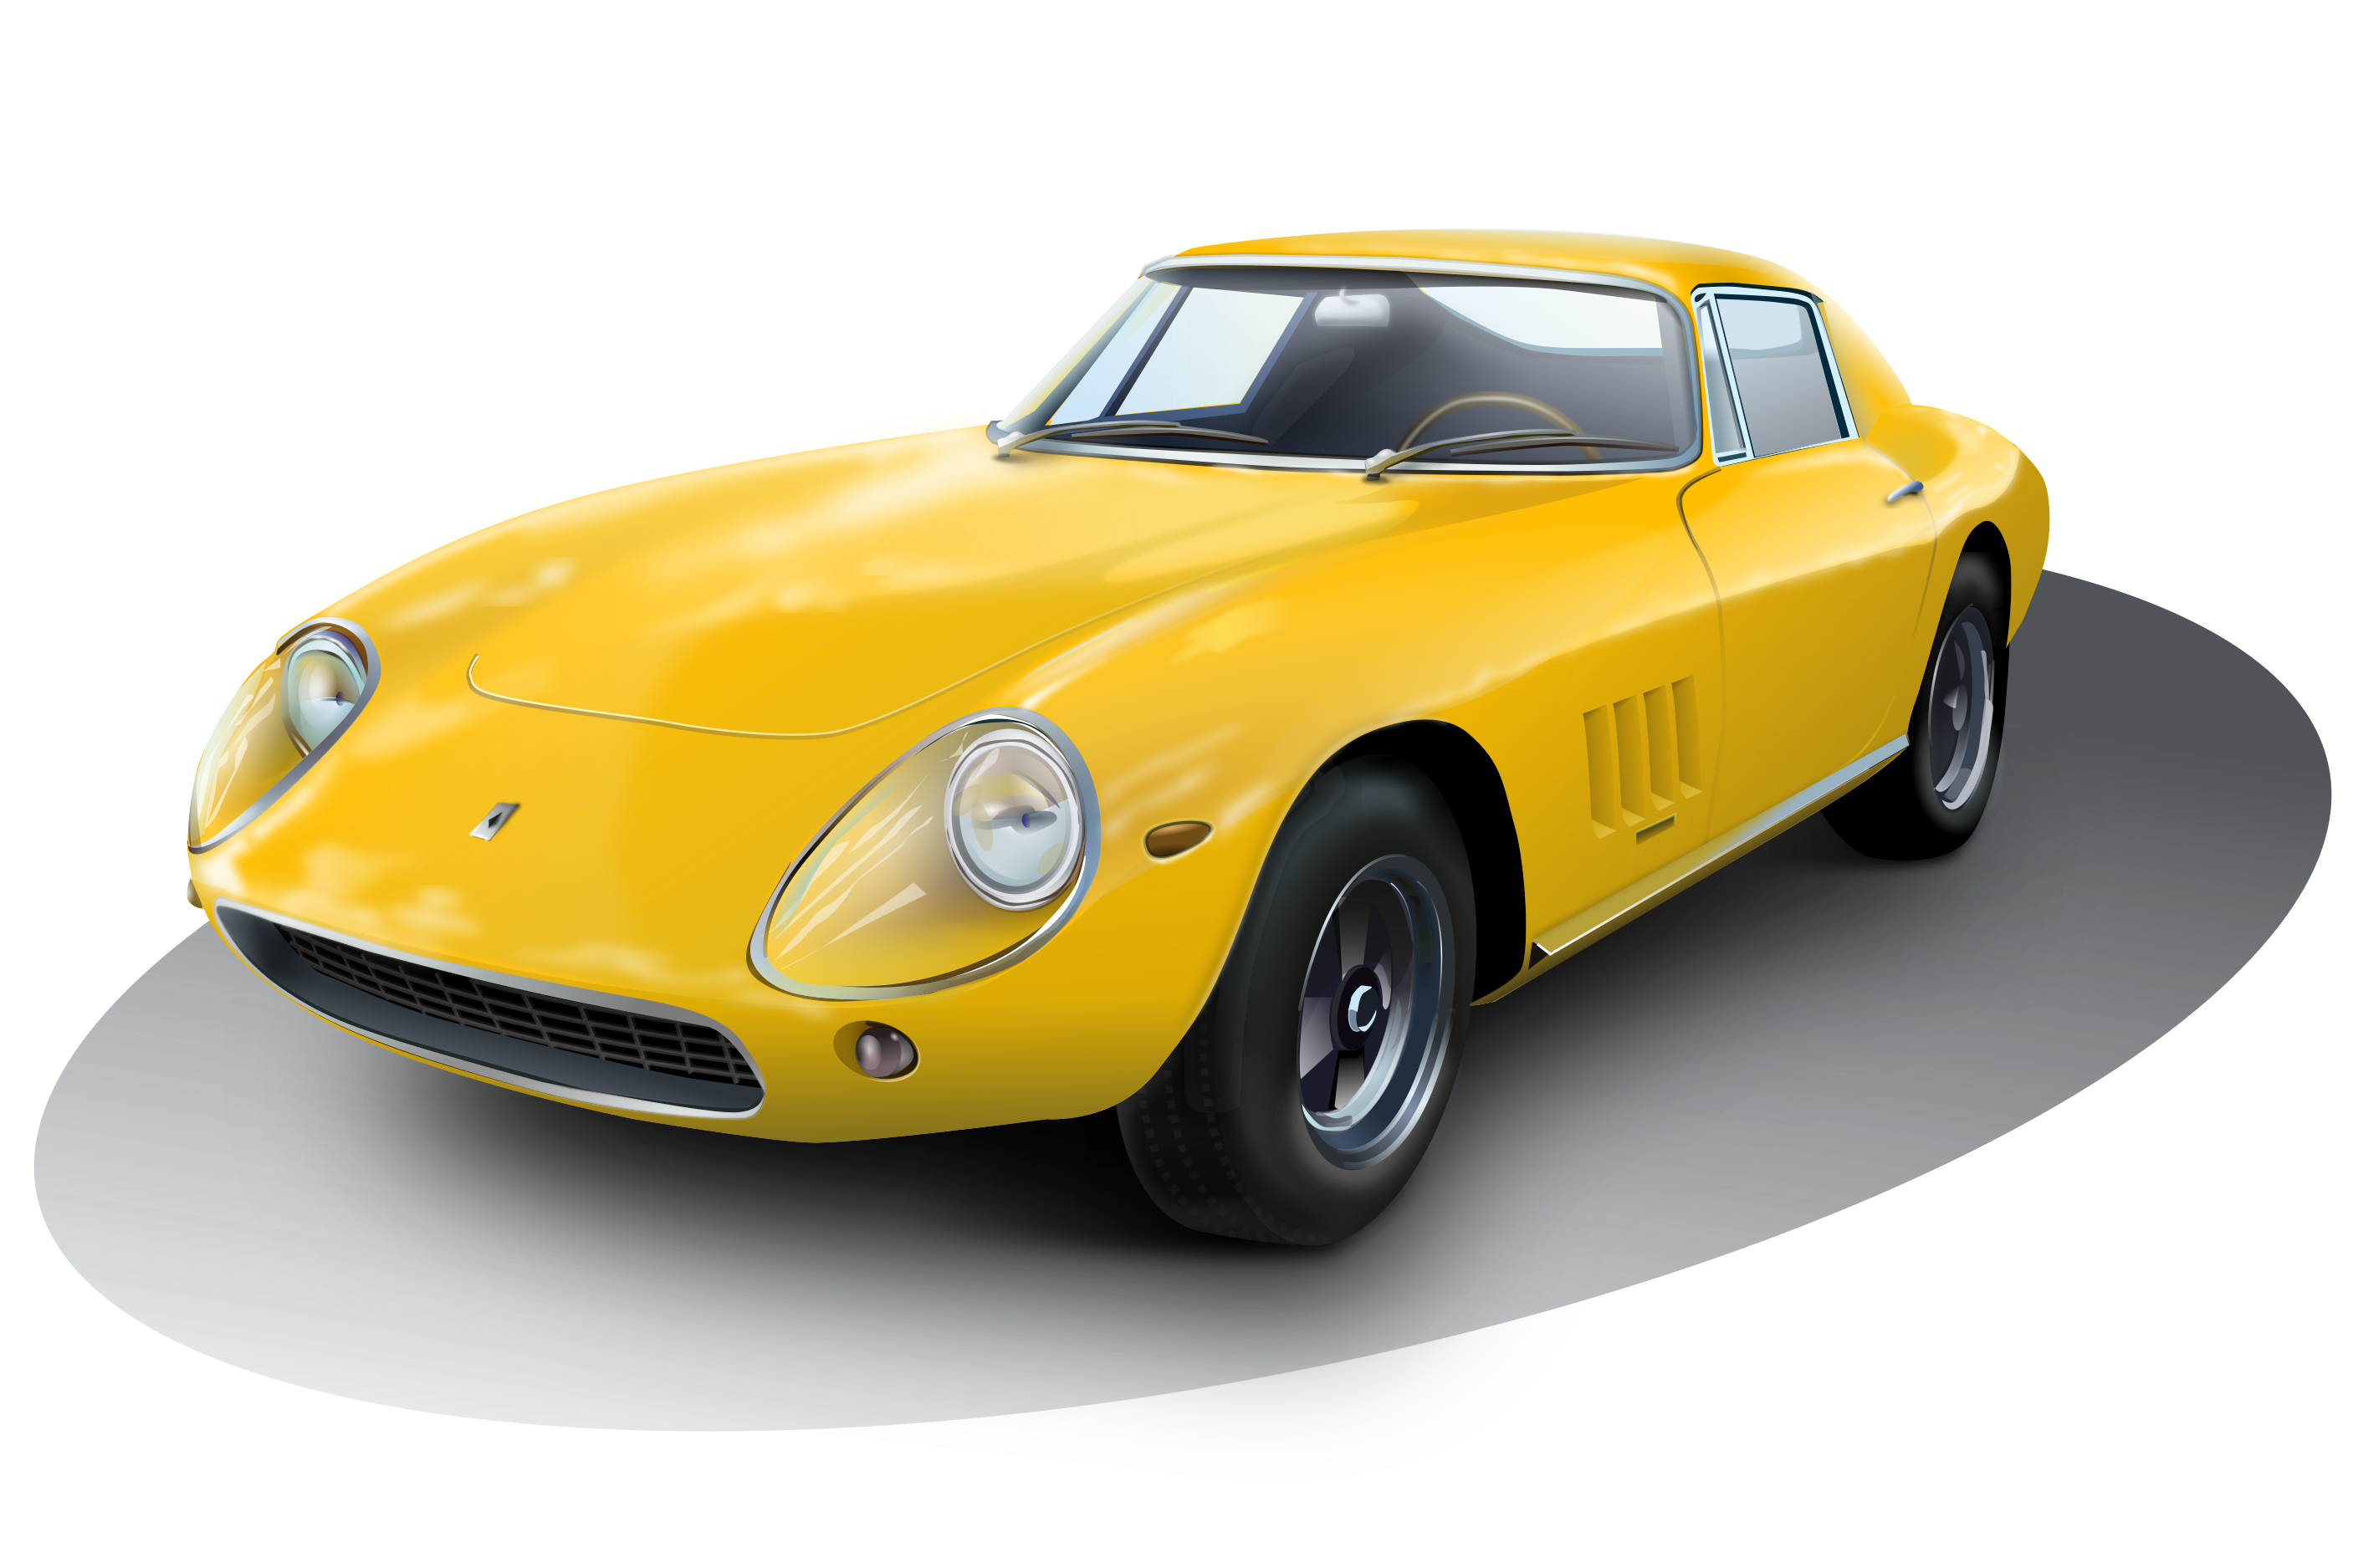
\includegraphics[scale=0.1]{Documeto/1-ElementosTextuais/1-Desenvolvimento/imagens-atividade1/car.png}

    \fonteElementoGrafico{Fornecido pelo Professor}
    
\end{figure}

\begin{figure}[h!]
    \centering
    \caption{Carro no formato SVG}
    \label{fig:carro_SVG}
    
    \includesvg[scale=0.1]{Documeto/1-ElementosTextuais/1-Desenvolvimento/imagens-atividade1/NewTux.svg}

    \fonteElementoGrafico{Fornecido pelo Professor}
    
\end{figure}

\hspace{1.5 cm} Escolheu-se essa imagem, pois, ela possui mais detalhes, o que a torna melhor para fazer esse tipo de comparação. Após converter a imagem para PNG já pode ser observado uma diferença, o tamanho da imagem aumentou quase 3,5$\times$. Depois, apenas as diferenças já explicitadas, a questão da perda de qualidade ao realizar o zoom. Para melhor exemplificar isso, seguem as Imagens \ref{fig:farol_carro_svg} e \ref{fig:farol_carro_png}.

\begin{figure}[h!]
    \centering
    \caption[Caption for LOF]{Farol do carro em SVG, zoom 500\% \footnotemark}
    \label{fig:farol_carro_svg}
    
    
\includegraphics[scale=0.7]{Documeto/1-ElementosTextuais/1-Desenvolvimento/imagens-atividade1/farol_car_svg.png}

    \fonteElementoGrafico{Fornecido pelo Professor}
    
\end{figure}
\footnotetext{Zoom renderizado no navegador \textit{Firefox}}

\begin{figure}[h!]
    \centering
    \caption[Caption for LOF]{Farol do carro em png, zoom 500\%\footnotemark}
    \label{fig:farol_carro_png}
    
    
\includegraphics[scale=0.3]{Documeto/1-ElementosTextuais/1-Desenvolvimento/imagens-atividade1/farol_car_png.png}

    \fonteElementoGrafico{Fornecido pelo Professor}
    
\end{figure}
\footnotetext{Zoom renderizado pelo aplicativo \textit{Photoshop}CS5 (obviamente obtido legalmente). Escolhemos esse \textit{software} para evitar filtros que outros aplicativos possam vir a utilizar ao dar zoom.}
    \captionsetup{justification=centering,margin=0cm}
\label{cap:atividade2}  % Forma de referenciar o capítulo no comando \ref

%inicio do capitulo
\chapter[Atividade 2 - Comparando diferentes subsamplings]{Atividade 2 - Comparando diferentes subsamplings}
Neste capítulo iremos realizar uma atividade um tanto um quanto peculiar, iremos utilizar o programa para análise de \textit{DownSampling}/\textit{SubSampling} em vídeo observando um arquivo sem compressão.

\section{Compreendendo melhor as informações fornecidas pelos arquivo}
Ao utilizar o software AvarexYUVPlayer com as seguintes configurações, evidenciadas na Figura \ref{fig:imagem8}:

\begin{figure}
    \centering
    \caption{Tela o software AvarexYUVPlayer}
    \label{fig:imagem8}
    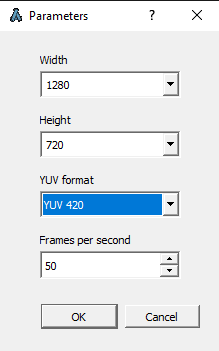
\includegraphics{Documeto/1-ElementosTextuais/images/08.png}

    \autoriaPropria
\end{figure}

\paragrafo Sendo o parâmetro de resolução crítico para visualização do video. Podemos analisar os efeitos do \textit{subsampling} em video, o que sinceramente alterou em nada na visualização do vídeo.

\paragrafo Ao tentar comprimir estes arquivos em RAR, ZIP e 7Z, foi-se obtidos resultados pouco satisfatórios, o ratio variou pouco entre os arquivos e esperávamos mais do 7Z, que exige um esforço computacional enorme e entrega algo ligeiramente melhor que os demais. Isto é, o ocorrido provavelmente se dá pelo software não ser capaz de aproveitar a pouca variação temporal, não tratam com eficiência vídeos no geral por conta disso.

obs: Não conseguimos fazer os cálculos para encontrar o valor exato do arquivo.


\section{Avaliando a influência dos parâmetros nos vídeos}
Em cada arquivo apenas varia o Subsampling, alterando “proporcionalmente” o tamanho do arquivo, mas sem alterar a qualidade, isso se deve ao fato de que subsampling é basicamente uma redução lossy de informações de luminância, informação essa que o ser humano não possui sensibilidade, passando despercebida. Além de que, por se tratar de um vídeo, é ainda mais complicado de perceber a diferença visto que não conseguimos analisar uma imagem por tempo o suficiente para separarmos as cores, causando uma mistura ainda maior e uma menor percepção de alterações de cores.
    \captionsetup{justification=centering,margin=0cm}
\label{cap:atividade3}  % Forma de referenciar o capítulo no comando \ref

%inicio do capitulo
\chapter[Atividade 3 - Analisando as características dinâmicas do vídeo]{Atividade 3 - Analisando as características dinâmicas do vídeo}

A seguinte atividade busca evidenciar a teoria através da prática. Ao analisarmos diferentes vídeos, com conteúdos, formatos e taxa de frames diferentes, pretende-se esclarecer onde a teoria encontra a prática.

\section{Vídeo 1 - Um vídeo em Slow Motion}
Pode-se abstrair um vídeo em slow motion como uma gravação a um FPS muito elevado exibido a um FPS baixo. Ou seja, suponha um vídeo gravado em 60 quadros por segundo. Se exibirmos ele a 30 quadros por segundo teremos a impressão de que as coisas estão mais lentas, isso porque um movimento que originalmente demoraria 1 segundo para ser concluído agora demora 2. É importante destacar isso, pois esse fato tem influência direta na redundância temporal do vídeo.

\paragrafo Como explicado pela teoria, a compressão de vídeo deve levar em consideração dois fatores: a redundância espacial e a redundância temporal. Em relação à redundância espacial, todos os conceitos de imagem são aplicados (afinal de contas, vídeos são compostos por imagens), ou seja, na redundância espacial busca-se comprimir uma imagem de uma forma inteligente o suficiente. No entanto, isso só é válido para os key frames, também chamados de quadros chave ou intra frames; nos demais, busca-se uma forma de otimizar o tamanho do vídeo. Para tal, uma série de técnicas são aplicadas a fim de aproveitar regiões que mantiveram-se estáticas para fazer a construção da próxima imagem.

\paragrafo Um vídeo em slow motion é perfeito para exemplificar a redundância temporal. Considerando o exemplo onde um movimento de 1 segundo é executado em 2 segundos, há uma maior suavidade no movimento. Assim, a distância entre um frame e outro é bem menor do que no caso original. Como pode ser observado na imagem abaixo, os vetores indicadores de movimento são muito pequenos, mesmo em cenas com grande movimentação.

\begin{figure}[H]
    \centering
    \caption{Imagem do vídeo em \textit{slowmotion}}
    \label{fig:imagem9}
    
    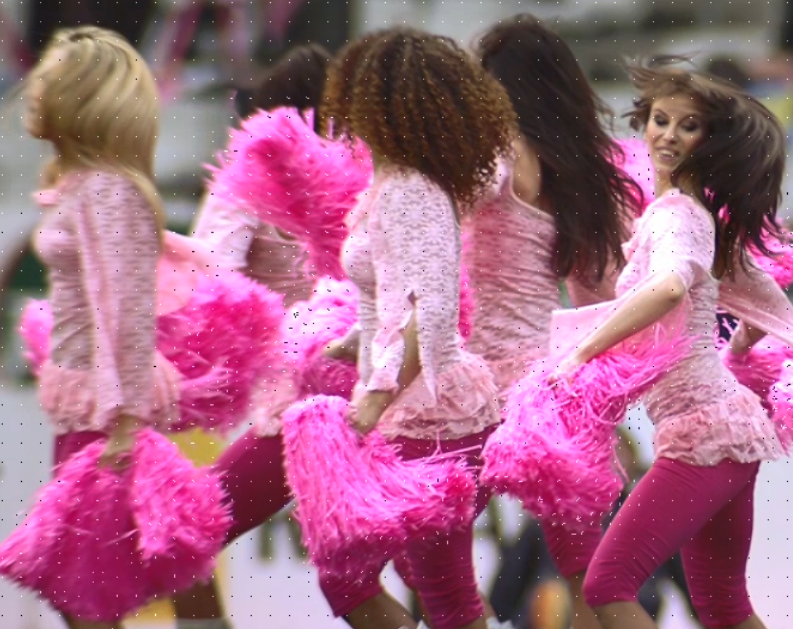
\includegraphics[scale=0.5]{Documeto/1-ElementosTextuais/images/09.png}

    \small
    Extraído dos vídeos fornecidos pelo Professor
\end{figure}

\paragrafo Outra coisa importante em relação a esse vídeo é a distribuição de frames do tipo I, B e P. No pseudo gráfico abaixo é possível identificar pontos de pico. Esses pontos de pico indicam quadros do tipo I. Como a composição do vídeo em slow motion é constituída por menos movimentos, o codec usa os I frames em momentos onde o acúmulo de perdas em relação a outros quadros é muito grande, ou em momentos específicos limitados por flags do arquivo. Repare que na maior parte do tempo, a segunda forma se faz verdadeira, mas há momentos, geralmente nas transições entre cenas, que o codec é obrigado a usar um frame tipo I para evitar maiores perdas.

\paragrafo Além disso, algo interessante ocorre no uso de quadros B e P. A proporção média é de um para um, isto é, um quadro P e um quadro B. Baseado nos nossos testes realizados de forma empírica, momentos de vídeos com maior redundância temporal costumam ter mais frames do tipo B do que a média se comparados a outros trechos do mesmo vídeo. No trecho do filme “The Matrix”, analisado na próxima sessão, há pouca presença de quadros B. No caso do arquivo em slow motion, a relação com a teoria encontrada foi que como a diferença entre um quadro no índice x em relação ao índice x+2 é tão pequena que a taxa de erro da composição também fica muito pequena, tornando viável seu uso do quadro tipo B no índice x+1.

\begin{figure}[H]
    \centering
    \caption{Imagem do vídeo em \textit{slowmotion}}
    \label{fig:imagem10}
    
    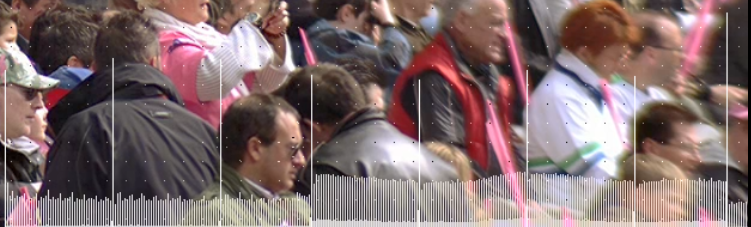
\includegraphics[scale=0.5]{Documeto/1-ElementosTextuais/images/10.png}

    \small
    Extraído dos vídeos fornecidos pelo Professor
\end{figure}

\paragrafo As informações importantes ainda não acabaram. O bitrate acompanha a complexidade da imagem analisada no momento, o que faz todo sentido. Sendo o bitrate a taxa de transferência de dados para a renderização do vídeo, faz sentido que imagens mais complexas exigirem uma maior taxa de transferência. No caso, os trechos mais pesados são os key frames, enquanto a complexidade dos demais é definida pela redundância temporal. Por exemplo, em cenas muito movimentadas, a tendência é que um bitrate maior seja exigido.

\section{Vídeo 2 - Cena Aleatória de The Matrix (1999)}

Boa parte das observações feitas na sessão anterior são válidas nesta sessão. No entanto, essa cena diferencia-se pela forma como foi gravada, que é no tempo normal. Além disso, a cena por si só é extremamente movimentada, com bolsa para lá e pra cá, tiro para todo lado, personagens andando, coadjuvantes morrendo, e zás e zás. Como pode-se perceber, a natureza da cena variou muito de uma análise para outra, assim é mais proveitoso interpretar as diferenças entre os vídeos do que ficar repetindo “mais do mesmo”.

\paragrafo A primeira coisa a se notar é que a imagem do vídeo em questão tem uma paleta de cores na cena mais escura e puxada para o verde se comparado ao vídeo em slow motion. Ou seja, a compressão da imagem é mais perceptível ao olho humano do que se a informação estivesse em regiões mais claras; o que implica na perda de transparência da imagem com mais facilidade. Isso influencia diretamente no bitrate necessário na descompressão. Isto é apenas um detalhe, mas não deixa de ser importante comentar.

\paragrafo Ademais, perceba que a quantidade de informação temporal dessa cena é muito maior do que a do vídeo em \textit{slowmotion}. A Figura \ref{fig:imagem11} demonstra isso com clareza. Nela, há uma vasta quantidade de \textit{motion vercotrs}, o que indica a movimentação das informações na cena, e por sua vez acumula informação. Isso influencia diretamente no bitrate, bem como na presença dos \textit{frames} tipo P e B.

\begin{figure}[H]
    \centering
    \caption{Imagem do filme \textit{The Matrix}}
    \label{fig:imagem11}
    
    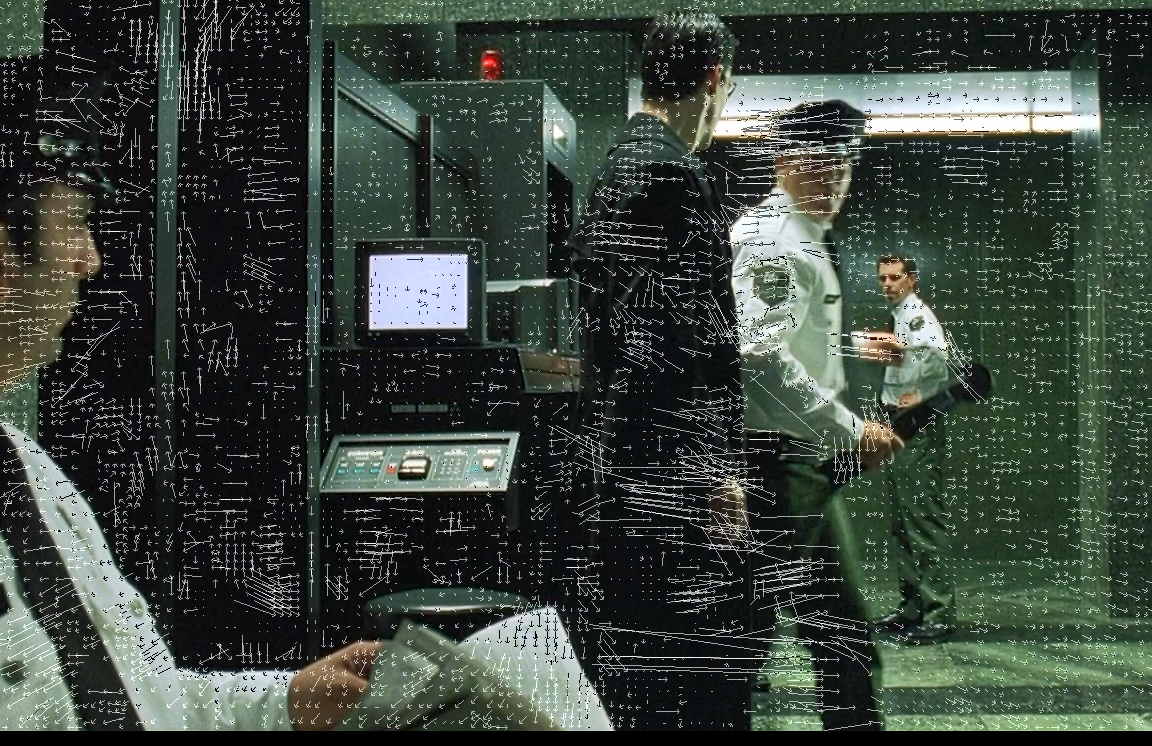
\includegraphics[scale=0.3]{Documeto/1-ElementosTextuais/images/11.png}

    \small
    Extraído dos vídeos fornecidos pelo Professor
\end{figure}

\paragrafo A Figura \ref{fig:imagem12} demonstra quais \textit{frames} o encoder optou por utilizar. Diferente do vídeo em \textit{slowmotion}, o trecho do filme não tão bem comportado. Os \textit{frames} tipo I não estão tão espaçados com a mesma constância que os \textit{frames} do vídeo anterior. Outra coisa que pode ser observadas é que esse tipo de quadro aparece em transições de cena. Além disso, há momentos de constância muito grande de frames tipo P, que são os momentos de uma "onda contínua", enquanto os \textit{frames} tipo B aparecem bem menos, em locais de "altura" menor. 

\begin{figure}[H]
    \centering
    \caption{Imagem do filme \textit{The Matrix}}
    \label{fig:imagem12}
    
    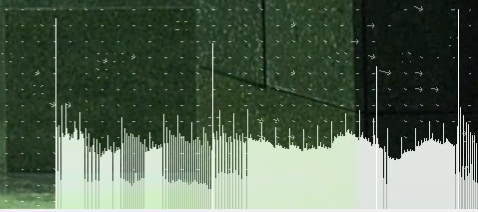
\includegraphics[scale=1]{Documeto/1-ElementosTextuais/images/12.png}

    \small
    Extraído dos vídeos fornecidos pelo Professor
\end{figure}


\section{Vídeo 3 - Último Episódio da Temporada 4 de \textit{Game of Thrones}}
Agora, é o momento de preparar uma pipoca e analisar um episódio longo de uma série mais longa ainda. Como o episódio é muito extenso não iremos comentar ele todo. Ao invés disso, vamos separar trechos interessantes de serem anualizados baseado nos conhecimentos então adquiridos.


\subsection{Um começo caótico}
Primeiramente, vamos analisar a tão famosa abertura da série. No primeiro momento, temos a logo da HBO Entretairement. Essa vinheta inicia-se com um ruído muito intenso, o que aumenta muito o bitrate nesse momento. Como demonstra a Figura \ref{fig:imagem12}, a construção da imagem é de alta complexidade espacial, apesar da pouca complexidade temporal.

\begin{figure}[H]
    \centering
    \caption{Imagens da abertura do episódio citado de \textit{Game of Trhones}}
    \label{fig:imagem13-14-15}
    
    
\includegraphics[scale=0.33]{Documeto/1-ElementosTextuais/images/13.png}
    
\includegraphics[scale=0.25]{Documeto/1-ElementosTextuais/images/14.png}

    \small
    Extraído dos vídeos fornecidos pelo Professor
\end{figure}

\paragrafo Então, a abertura da série é exibida e ela tem, de forma geral, uma complexidade bem maior que o resto do episodio, já que o seu \textit{bitrate} foi consideravelmente maior que a média. Isso ocorre devido a dois fatores: primeiro, a complexidade espacial dela é bem grande, com muitas formas bem definidas e regiões com bastante "textura"; a segunda é que a complexidade temporal em toda a cena é bastante constate -- geralmente, uma cena pode ter complexidade temporal alta, mas costuma ser em pontos específicos na tela, ou no cenário ou em um objeto, já na abertura a cena como um todo tem movimento.


\subsection{Cenas escuras}
A Figura \ref{fig:imagem17} traz outra cena do episódio. Enquanto a abertura era bem mais complexa, esse trecho é mais simples. Apesar da correção de movimento ser muito intensa, a forma como a câmera constrói a cena permite muita redundância nas informações.

\begin{figure}[H]
    \centering
    \caption{Imagem do início do episódio citado de \textit{Game of Trhones}}
    \label{fig:imagem17}
    
    
\includegraphics[scale=0.35]{Documeto/1-ElementosTextuais/images/17.png}

    \small
    Extraído dos vídeos fornecidos pelo Professor
\end{figure}

\paragrafo Além disso, cenas que tem um ritmo mais lento tem um gráfico de complexidade mais comportado. Em comparação a cenas mais claras, os artefatos são muito evidentes nos trechos mais escuros, como demonstrado na Figura \ref{fig:imagem18}

\begin{figure}[H]
    \centering
    \caption{Imagem do episódio citado de \textit{Game of Trhones}}
    \label{fig:imagem18}
    
    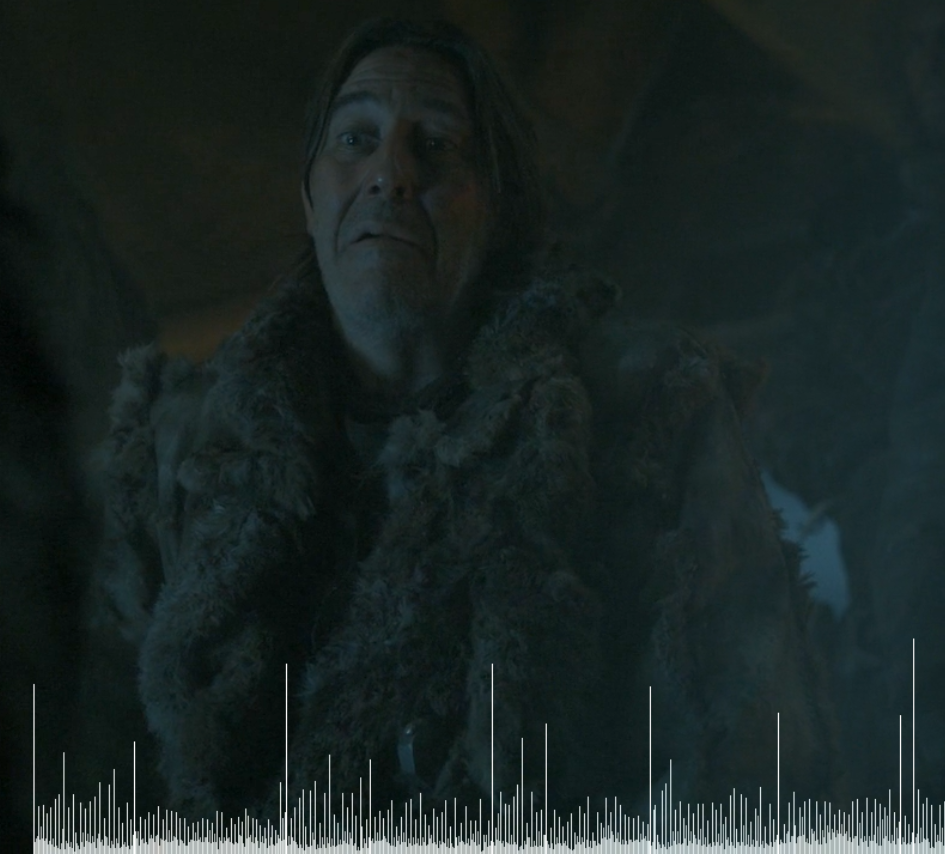
\includegraphics[scale=0.35]{Documeto/1-ElementosTextuais/images/18.png}

    \small
    Extraído dos vídeos fornecidos pelo Professor
\end{figure}


\subsection{Cenas Claras}
Em cenas claras um comportamento semelhante pode ser observado. Regiões mais escuras tem artefatos bastante visíveis, enquanto regiões mais claras são mais transparentes. Além disso, momentos mais calmos apresentam gráficos mais comportados.

\begin{figure}[H]
    \centering
    \caption{Imagem do episódio citado de \textit{Game of Trhones}}
    \label{fig:imagem19}
    
    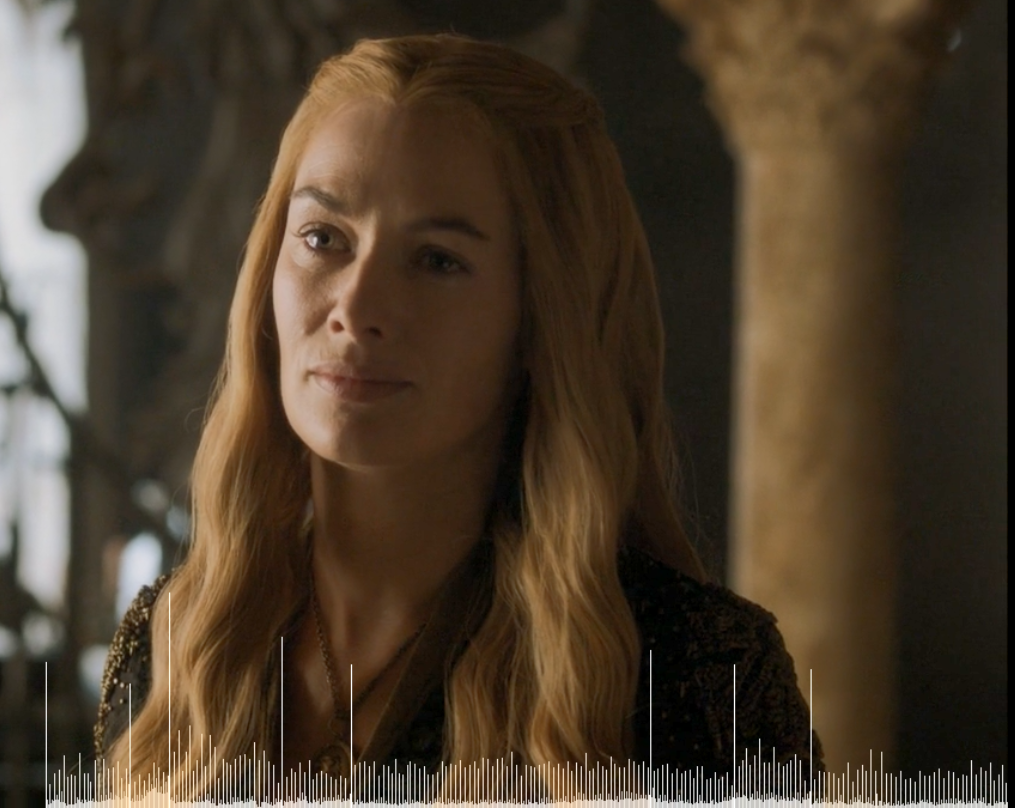
\includegraphics[scale=0.35]{Documeto/1-ElementosTextuais/images/19.png}

    \small
    Extraído dos vídeos fornecidos pelo Professor
\end{figure}

\paragrafo Além disso, é muito interessante perceber como a iluminação artificial e a iluminação natural tem grande influência na percepção dos artefatos e também no comportamento da complexidade da cena. Quando a iluminação é artificial, os artefatos são mais perceptíveis e a transição entre camadas é bem mais suave, valorizando a cena. Além disso, em cenas com iluminação artificial é comum perceber que há uma variância muito brusca na correção de movimento mesmo que as personagens estejam paradas, o que é justificado pelo fato da iluminação artificial "piscar" ao invés de emitir de fato luz.


\begin{figure}[H]
    \centering
    \caption{Imagem do episódio citado de \textit{Game of Trhones} (supostamente em iluminação artificial); a imagem da direita é o exato frame posterior ao frame da esquerda}
    \label{fig:imagem20-21}
    
    
\includegraphics[scale=0.3]{Documeto/1-ElementosTextuais/images/20.png}
    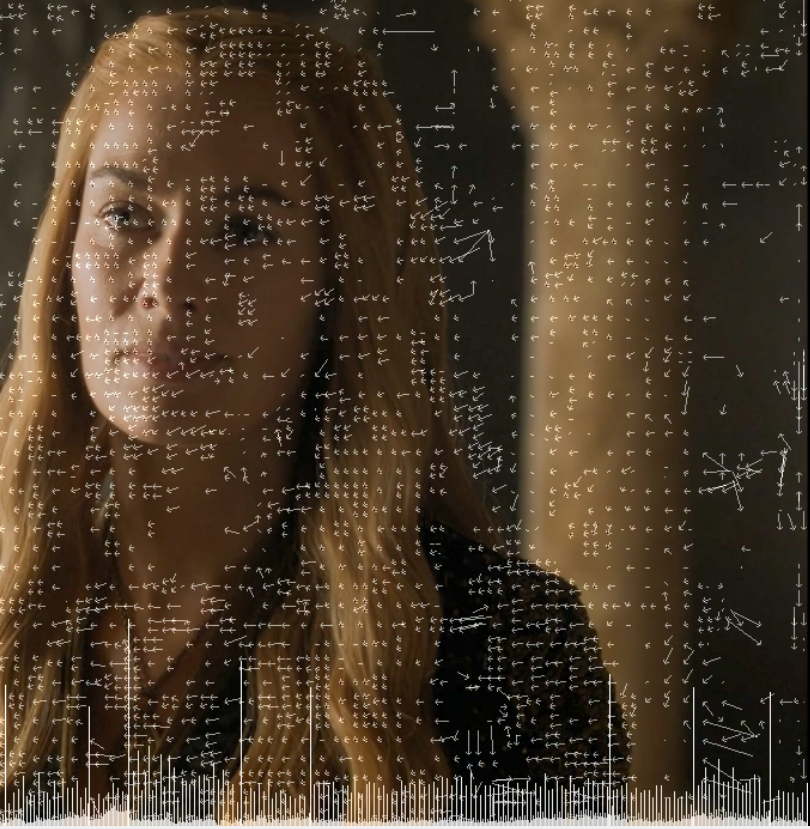
\includegraphics[scale=0.3]{Documeto/1-ElementosTextuais/images/21.png}

    \small
    Extraído dos vídeos fornecidos pelo Professor
\end{figure}


\begin{figure}[H]
    \centering
    \caption{Imagem do episódio citado de \textit{Game of Trhones} (supostamente em iluminação natural); a imagem da direita é o exato frame posterior ao frame da esquerda}
    \label{fig:imagem22-23}
    
    
\includegraphics[scale=0.3]{Documeto/1-ElementosTextuais/images/22.png}
    
\includegraphics[scale=0.3]{Documeto/1-ElementosTextuais/images/23.png}

    \small
    Extraído dos vídeos fornecidos pelo Professor
\end{figure}

\subsection{Cenas mais calmas com alta complexidade}
Existem cenas que mesmo que sejam bem lentas, a sua complexidade é muito grande. Isso decorre do fato da complexidade temporal ser baixa, mas da espacial ser grande. No episódio, próximo ao final dele, temos uma cena em uma região montanhosa. Como é de se esperar, essa cena tem bastante textura, muitos detalhes e também camadas. Assim, a sua complexidade espacial é bastante alta.

\begin{figure}[H]
    \centering
    \caption{Imagem do episódio citado de \textit{Game of Trhones}}
    \label{fig:imagem24}
    
    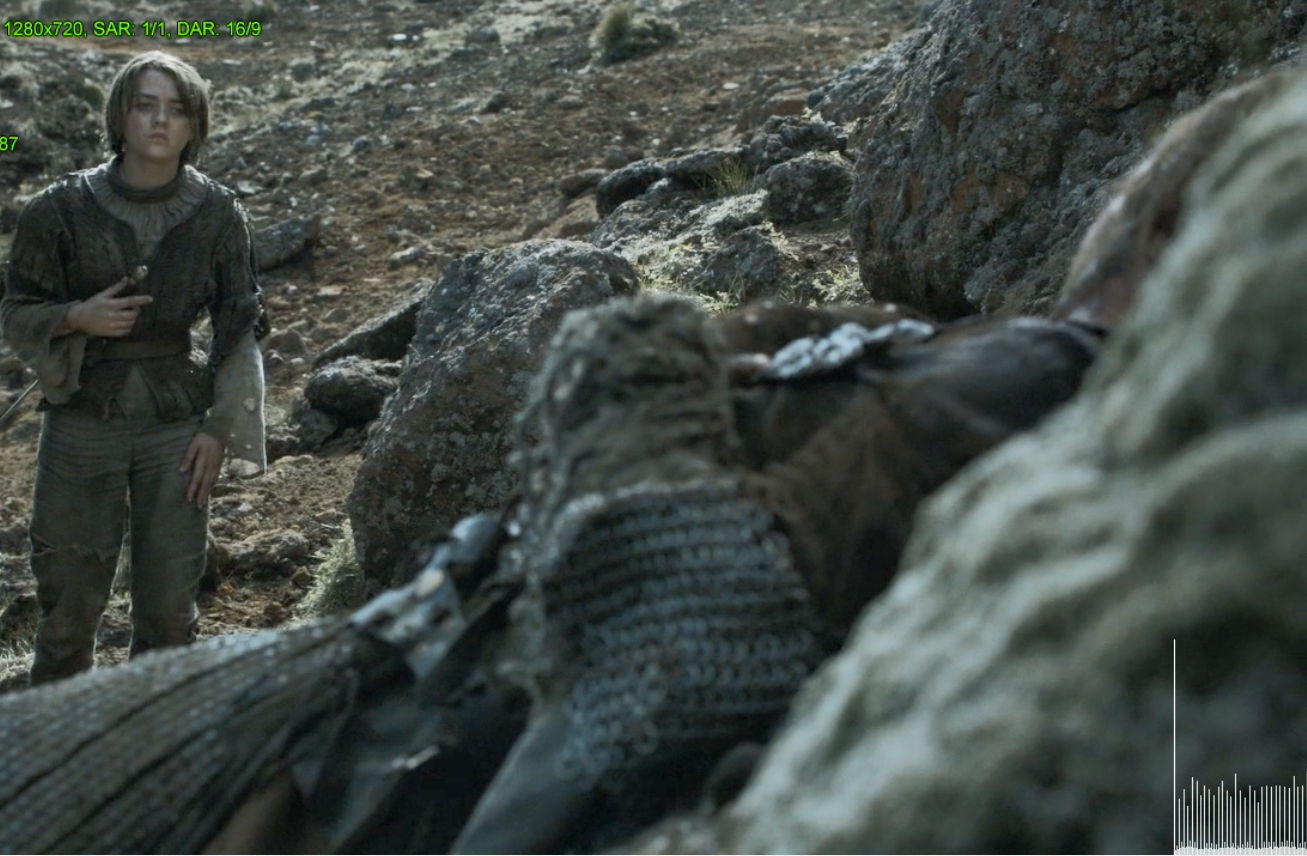
\includegraphics[scale=0.3]{Documeto/1-ElementosTextuais/images/24.png}

    \small
    Extraído dos vídeos fornecidos pelo Professor
\end{figure}
    \captionsetup{justification=centering,margin=0cm}
\label{cap:atividade4}  % Forma de referenciar o capítulo no comando \ref

%inicio do capitulo
\chapter[Atividade 4 - Conversão de vídeo]{Atividade 4 - Conversão de vídeo}

A fim de descobrir as nuances de dois formatos de vídeo x264, x265, AV1 e suas diferenças, a próxima atividade revelará resultados oriundos de uma série de testes para identificar parâmetros para um vídeo considerado bom (transparente) e um ruim (tolerável). Os vídeos utilizados nessa tarefa foram: Big Bunk Bunny e Tears Of Steel.

\section{Atividade 4A - Comprimindo para H.264/AVC}
Irei partir do formato mais antigo e ainda muito utilizado ainda nos dias de hoje, o x264, os resultados serão expostos a seguir.

\paragrafo Big Bunk Bunny: Neste vídeo, iniciei testando o extremo da compressão, gerando um resultado péssimo como esperado. Na tentativa de achar algo transparente, cheguei em 28,5 como fator de qualidade com \textit{bitrate} médio de 1.714Kbps. Enquanto que para algo tolerável, aos olhos bem treinados, a partir de 37, com bitrate médio de 779Kbps. A partir deste ponto o vídeo começa a dar desconforto ao assistir, sendo possível estender até um máximo de 39, que é quando a qualidade fica muito ruim.

\paragrafo Tearls Of Steel: Aqui seguimos a mesma lógica da anterior entretanto o grau de transparência é alcançado até 30, bitrate de 1.623Kbps, e de tolerância em 38, bitrate de 841Kbps, e apesar de possuir um fator maior em comparação ao outro vídeo, no fator máximo ele incomoda consideravelmente mais. 

\paragrafo No geral, a compressão dos vídeos foram rápidas, demorando em média apenas 3 minutos para os vídeos. A Tabela \ref{tab:tabela4a} exibe o Tamanho, bitrate e ratio de cada compressão a fim de melhorar a visualização dos dados.

\begin{table}[H]
    \centering
    \caption{Tabela 4 A}
    \label{tab:tabela4a}
    \begin{tabularx}{\textwidth}{X|C|C|C|C|C|C}
        \hline
        \textbf{Vídeo} & \textbf{Original} & \textbf{Lossless} & \textbf{Lossy} & \textbf{Bitrate Medio (kpbs)} & \textbf{Ratio (original)} & \textbf{Ratio (lossless)} \\ \hline
        Big Buck Bunny (HQ) & 42.462,79 & 10.524,19 & 121,9 & 1714 & 0,00287 & 0,01158 \\ \hline
        Tears Of Steel (HQ) & 44.256,58 & 13.359,21 & 142 & 1623 & 0,00321 & 0,01063 \\ \hline
        Big Buck Bunny (LQ) & 42.462,79 & 10.524,19 & 55,42 & 779 & 0,00131 & 0,01158 \\ \hline
        Tears Of Steel (LQ) & 44.256,58 & 13.359,21 & 73,57 & 841 & 0,00166 & 0,01063 \\ \hline
    \end{tabularx}

    \autoriaPropria
\end{table}


\paragrafo Partindo para uma comparação de eficiência entre CPU e GPU para compressão de vídeo. Na ocasião é uma disputa entre rx580 , que é uma placa gráfica já antiga, e um xeon, que possui muitos núcleos atuando em um programa muito paralelizado, tornando uma disputa relativamente equilibrada. Abaixo a Tabela \ref{tab:tabela4a-continuação} exibe o FPS médio do processo.

\begin{table}[H]
    \centering
    \caption{Tabela 4 A - Continuação}
    \label{tab:tabela4a-continuação}
    \begin{tabularx}{\textwidth}{X|C|C}
        \hline
        \multicolumn{3}{c}{\textbf{FPS}} \\ \hline
        \textbf{Vídeo} & \textbf{h264} & \textbf{VCE h264} \\ \hline
        Tears Of Steel & 107,1 & 124,2 \\ \hline
        Big Buck Bunny & 106,5 & 112,5 \\ \hline
    \end{tabularx}

    \autoriaPropria
\end{table}

\paragrafo Apesar da GPU ter grande vantagem por ser especializada em calculo de matrizes, a CPU possui muitos núcleos para compensar, de maneira a ser muito eficiente para compressão, criando uma diferença consideravelmente pequena entre eles dada sua otimização para tarefa.

\section{Atividade 4B - Comprimindo para H.265/HEVC}
Agora partindo para o próximo formato, o h265. Teoricamente ele possui uma melhor qualidade de compressão, apesar de ser um pouco mais custoso computacionalmente, é isso que iremos observar a partir de agora.

\paragrafo Big Bunk Bunny: Se realmente houveram melhorarias em relação à sua versão an terior, não sabemos dizer só com estes testes, entretanto o formato ainda pesa na compressão, trazendo artefatos e má qualidade com facilidade se não prestar atenção no fator qualidade. Para vídeos transparentes, foi encontrado o fator 26 com \textit{bitrate} de 1708 kbps. Variando um pouco esses parâmetros, obtém-se um vídeo tolerável até o fator 30 com \textit{bitrate} de 1096 kbps; com uma compressão mais abrupta, a qualidade da imagem passa a ser um grande incômodo.

\paragrafo Tearls Of Steel: Aqui serei mais direto, fator qualidade 27,5 para transparente e 32 o tolerável com bitrate de 1596 e 868 respectivamente.

\paragrafo Este formato demorar pouco mais para processar os vídeos, pouco menos de 5 minutos cada, a qualidade é boa com um tamanho/\textit{bitrate} realmente otimizado. As Tabelas \ref{tab:tabela4b} e \ref{tab:tabela4b-continuação} trazem informações detalhadas dos testes, permitindo uma comparação mais específica.

%bunny
%transparente 26
%toleravel 30
%steel
%transparente 27,5
%toleravel 32

\paragrafo 

\begin{table}[H]
    \centering
    \caption{Tabela 4 B}
    \label{tab:tabela4b}
    \begin{tabularx}{\textwidth}{X|C|C|C|C|C|C}
        \hline
        \textbf{Vídeo} & \textbf{Original} & \textbf{Lossless} & \textbf{Lossy} & \textbf{Bitrate Medio (kpbs)} & \textbf{Ratio (original)} & \textbf{Ratio (lossless)} \\ \hline
        Big Buck Bunny (HQ) & 42.462,79 & 10.524,19 & 121,43 & 1708 & 0,00286 & 0,01154 \\ \hline
        Tears Of Steel (HQ) & 44.256,58 & 13.359,21 & 139,67 & 1596 & 0,00316 & 0,01045 \\ \hline
        Big Buck Bunny (LQ) & 42.462,79 & 10.524,19 & 77,94 & 1096 & 0,00184 & 0,00741 \\ \hline
        Tears Of Steel (LQ) & 44.256,58 & 13.359,21 & 75,99 & 868 & 0,00172 & 0,00569 \\ \hline
    \end{tabularx}

    \autoriaPropria
\end{table}

\begin{table}[H]
    \centering
    \caption{Tabela 4 B - Continuação}
    \label{tab:tabela4b-continuação}
    \begin{tabularx}{\textwidth}{X|C|C}
        \hline
        \multicolumn{3}{c}{\textbf{FPS}} \\ \hline
        Vídeo & h265 & VCE h265 \\ \hline
        Tears Of Steel & 63,6 & 121,4 \\ \hline
        Big Buck Bunny & 66,4 & 112,5 \\ \hline
    \end{tabularx}

    \autoriaPropria
\end{table}

\section{Atividade 4C - Comprimindo para AV1}
Finalmente alcançamos o ultimo formato e mais pesado computacionalmente entre eles, trazendo (teoricamente) uma ótima qualidade, afinal, grandes empresas estão por traz dele. Para melhor dinamismo irei apresentar apenas as tabelas e o restante é fácil de explicar.

\begin{table}[H]
    \centering
    \caption{Tabela 4 C}
    \label{tab:tabela4C}
    \begin{tabularx}{\textwidth}{X|C|C|C|C|C|C}
        \hline
        \textbf{Vídeo} & \textbf{Original} & \textbf{Lossless} & \textbf{Lossy} & \textbf{Bitrate Medio (kpbs)} & \textbf{Ratio (original)} & \textbf{Ratio (lossless)} \\ \hline
        Big Buck Bunny (HQ) & 42.462,79 & 10.524,19 & 57,63 & 810 & 0,00136 & 0,00548 \\ \hline
        Tears Of Steel (HQ) & 44.256,58 & 13.359,21 & 128,53 & 1469 & 0,00290 & 0,00962 \\ \hline
        Big Buck Bunny (LQ) & 42.462,79 & 10.524,19 & 26,85 & 378 & 0,00063 & 0,00255 \\ \hline
        Tears Of Steel (LQ) & 44.256,58 & 13.359,21 & 33,08 & 378 & 0,00075 & 0,00248 \\ \hline
    \end{tabularx}

    \autoriaPropria
\end{table}

\begin{table}[H]
    \centering
    \caption{Tabela 4 C - Continuação}
    \label{tab:tabela4c-continuação}
    \begin{tabularx}{\textwidth}{XC}
        \hline
        \multicolumn{2}{c}{\textbf{FPS}} \\ \hline
        Vídeo & VCE AV1 \\ \hline
        Tears Of Steel & 10,9 \\
        Big Buck Bunny & 10,3 \\ \hline
    \end{tabularx}

    \autoriaPropria


\end{table}

\paragrafo Em Big Buck Bunny, o fator de qualidade transparente é 52 e tolerante 63, enquanto para Tears Of Steel os valores são 53 e 63 respectivamente. Quanto a questão do esforço computacional, imaginei que seria demasiado custoso, entretanto não tanto. Um video com Enconder Preset 3, demorou em média 33 minutos para finalizar, enquanto o mesmo com 4 mudou o tempo para 25, o tornando possivelmente inviável para quantidades massivas de vídeos sem uma máquina potente o suficiente ou especializada para a tarefa.


%bunny
%transparente 52
%toleravel 63
%steel
%transparente 53
%toleravel 63

\section{Atividade 4D - Avaliação geral do desempenho dos formatos}
Agora é o momento de comparar os diferentes codecs. Isso é particularmente importante para acompanharmos a evolução dos algoritmos. Todos os arquivos podem ser acessados no link \url{https://drive.google.com/drive/folders/160xDMlNdiJo1Q8intSz2KlbsdiY7OROl}.

\paragrafo O h.264 foi competente em sua função. Apesar da nítida baixa qualidade, o vídeo pode ser assistido sem muitos prejuízos e a sua codificação é bem rápida, se tornando viável para quem não quer muita dor de cabeça com vídeos. No entanto, o h.265 não nos impressionou tanto. Há uma evolução considerável em relação ao h.264, qualidade melhor de imagem, menor presença de artefato, dentre outras vantagens. No entanto, ele deixou a desejar no sentido da velocidade e na taxa de compressão. Pela Tabelas abaixo, podemos observar que a taxa média de compressão foi de, somente, 0,61\%, um resultado quase ínfimo, entretando, inegavelmente com uma qualidade pouco superior.

\paragrafo Em relação ao AV1, esse sim nos impressionou. Se comparado ao h.265 o arquivo também não é tão menor, mas a qualidade da imagem é muito superior. Os artefatos aparecem deforma reduzida e mesmo parâmetros pouco otimizados são suficientes. Digamos que é preciso fazer "muita besteira" para o vídeo ficar ruim.

\paragrafo Nos formatos de vídeo em que se utiliza o hardware, a compressão deixou muito a desejar, demonstrando resultados ruins.


\begin{table}[H]
    \centering
    \caption{Tabela 4 D}
    \label{tab:tabela4d}
    \footnotesize
    \begin{tabularx}{\textwidth}{X|C|C|C|C|C|C|C|C|C}
        \hline
        
        Vídeo & Original & Lossless & Tamanho & Bitrate Medio (kpbs) & Fator de Quali- dade & Velocidade de Compres- são & Ratio (\%) [Arquivo / Original] & Ratio (\%) [Arquivo / Lossless] & Ratio (\%) [Arquivo / h.264] \\ \hline
        Big Buck Bunny h.264HQ & 42.462,79 & 10.524,19 & 121,90 & 1.714,00 & 28,50 & 107,1 & 0,29\% & 1,16\% & - \\ \hline
        Big Buck Bunny h.264LQ & 42.462,79 & 10.524,19 & 55,42 & 779,00 & 37,00 & - & 0,13\% & 0,53\% & - \\ \hline
        Big Buck Bunny h.264 VCE HQ & 42.462,79 & 10.524,19 & 505,00 & 7.104,00 & 28,50 & 124,2 & 1,19\% & 4,80\% & - \\ \hline
        Big Buck Bunny h.265HQ & 42.462,79 & 10.524,19 & 57,63 & 810,00 & 26,00 & 63,60 & 0,14\% & 0,55\% & 0,47 \\ \hline
        Big Buck Bunny h.265LQ & 42.462,79 & 10.524,19 & 26,85 & 378,00 & 30,00 & - & 0,06\% & 0,26\% & 0,48 \\ \hline
        Big Buck Bunny h.265 VCE HQ & 42.462,79 & 10.524,19 & 263,00 & 3.710,00 & 26,00 & 121,40 & 0,62\% & 2,50\% & 0,52 \\ \hline
        Big Buck Bunny AV1 HQ & 42.462,79 & 10.524,19 & 121,43 & 1.708,00 & 52,00 & - & 0,29\% & 1,15\% & 1,00 \\ \hline
        Big Buck Bunny AV1 LQ & 42.462,79 & 10.524,19 & 77,94 & 1.096,00 & 63,00 & - & 0,18\% & 0,74\% & 1,41 \\ \hline
    \end{tabularx}

    \autoriaPropria
\end{table}


\begin{table}[H]
    \centering
    \caption{Tabela 4 D}
    \label{tab:tabela4d}
    \footnotesize
    \begin{tabularx}{\textwidth}{X|C|C|C|C|C|C|C|C|C}
        \hline
        
        Vídeo & Original & Lossless & Tamanho & Bitrate Medio (kpbs) & Fator de Quali- dade & Velocidade de Compres- são & Ratio (\%) [Arquivo / Original] & Ratio (\%) [Arquivo / Lossless] & Ratio (\%) [Arquivo / h.264] \\ \hline
        Tears Of Steel h.264HQ & 44.256,58 & 13.359,21 & 142,00 & 1.623,00 & 30,00 & 106,5 & 0,32\% & 1,06\% & - \\ \hline
        Tears Of Steel h.264LQ & 44.256,58 & 13.359,21 & 73,57 & 841,00 & 38,00 & - & 0,17\% & 0,55\% & - \\ \hline
        Tears Of Steel h.264 VCE HQ & 44.256,58 & 13.359,21 & 389,00 & 4.456,00 & 30,00 & 112,5 & 0,88\% & 2,91\% & - \\ \hline
        Tears Of Steel h.265HQ & 44.256,58 & 13.359,21 & 128,53 & 1.469,00 & 27,50 & 66,40 & 0,29\% & 0,96\% & 1,05 \\ \hline
        Tears Of Steel h.265LQ & 44.256,58 & 13.359,21 & 33,08 & 378,00 & 32,00 & - & 0,07\% & 0,25\% & 0,60 \\ \hline
        Tears Of Steel h.265 VCE HQ & 44.256,58 & 13.359,21 & 275,00 & 3.150,00 & 27,50 & 112,50 & 0,62\% & 2,06\% & 0,54 \\ \hline
        Tears Of Steel AV1 HQ & 44.256,58 & 13.359,21 & 139,67 & 1.596,00 & 53,00 & 10,9 & 0,32\% & 1,05\% & 1,15 \\ \hline
        Tears Of Steel AV1 LQ & 44.256,58 & 13.359,21 & 75,99 & 868,00 & 63,00 & 10,30 & 0,17\% & 0,57\% & 1,37 \\ \hline
    \end{tabularx}


\end{table}
        


    % ----------------------------------------------------------

\captionsetup{justification=centering,margin=0cm}

%inicio do capitulo
\chapter[CONCLUSÃO]{CONCLUSÃO}
\index{CONCLUSÃO}
\label{cap:conclusão}

Após a finalização do trabalho uma série de conhecimentos puderam ser absorvidos. Não só conteúdos importantes para a nossa formação profissional e acadêmica bem como para a nossa vida mesmo. Otimizar o espaço de um hd, escolher a melhor formato de armazenar vídeos, escolher a melhor forma para gravar os vídeos (afinal de constas, se formos subir um vídeo em uma plataforma é melhor que ele seja feito na melhor qualidade para evitar compressões muito desastrosas). Além disso, nossas vidas jamaisserão as mesmas, pois diferente de imagens, os vídeos estão sempre com perdas. Ou seja, cada vídeo no youtube é igual a um ano de vida a menos. 

\url{https://youtu.be/1d_RleeOSyM}



\end{document}